\usetikzlibrary{arrows.meta,calc}
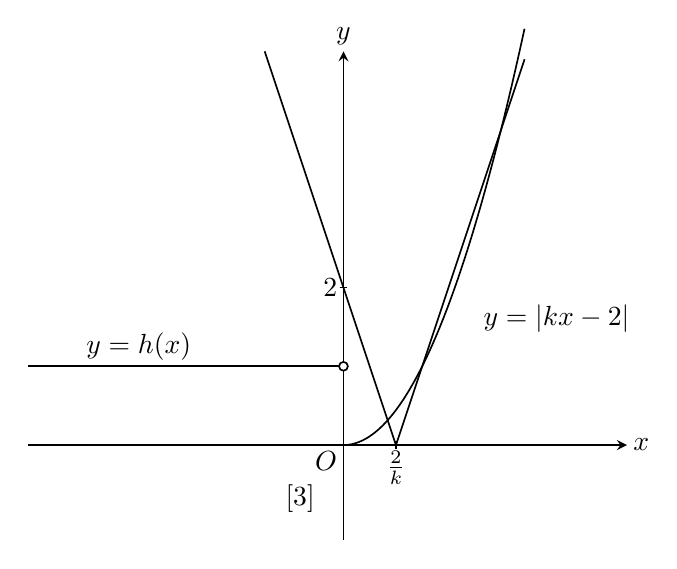
\begin{tikzpicture}[x=1cm,y=1cm,line width=.6pt,>=stealth]
\draw[->] (-4.0,0)--(3.6,0) node[right,inner sep=0pt,xshift=2pt] {$x$};
\draw[->] (0,-1.2)--(0,5.0) node[above,inner sep=0pt,yshift=2pt] {$y$};
\draw (-0.05,2)--(0.05,2);
\node[left,inner sep=0pt,xshift=-2pt] at (0,2) {$2$};
\draw (0.6667,-0.05)--(0.6667,0.05);
\node[below,inner sep=0pt,yshift=-2pt] at (0.6667,0) {$\frac{2}{k}$};
\node[below left,inner sep=0pt,xshift=-2pt,yshift=-2pt] at (0,0) {$O$};
\draw[domain=-4.0:0,samples=2] plot (\x,{1});
\draw[fill=white] (0,1) circle (1.6pt);
\draw[domain=0:2.3,samples=100] plot (\x,{\x*\x});
\draw[domain=-1.0:0.6667,samples=2] plot (\x,{abs(3*\x-2)});
\draw[domain=0.6667:2.3,samples=2] plot (\x,{abs(3*\x-2)});
\node[above,inner sep=0pt,yshift=2pt] at (-2.6,1) {$y=h(x)$};
\node[right,inner sep=0pt,xshift=2pt] at (1.7,1.6) {$y=|kx-2|$};
\node[below,inner sep=0pt,yshift=-14pt] at (-0.55,0) {\bitmapinsertcaption[3]};
\end{tikzpicture}
